\documentclass[UTF8]{ctexart}

\usepackage{listings}
\usepackage{xcolor}
\usepackage{tikz}
\definecolor{mygreen}{rgb}{0,0.6,0}
\definecolor{mygray}{rgb}{0.5,0.5,0.5}
\definecolor{mymauve}{rgb}{0.58,0,0.82}


\lstset{ %
    backgroundcolor=\color{white},  % choose the background color; you must add \usepackage{color} or \usepackage{xcolor}
    basicstyle=\footnotesize,       % the size of the fonts that are used for the code
    breakatwhitespace=false,        % sets if automatic breaks should only happen at whitespace
    breaklines=true,                % sets automatic line breaking
    captionpos=bl,                  % sets the caption-position to bottom
    commentstyle=\color{gray},      % comment style
    extendedchars=true,             % lets you use non-ASCII characters; for 8-bits encodings only, does not work with UTF-8
    frame=single,                   % adds a frame around the code
    keepspaces=true,                % keeps spaces in text, useful for keeping indentation of code (possibly needs columns=flexible)
    keywordstyle=\color{purple},    % keyword style
    numbers=left,                   % where to put the line-numbers; possible values are (none, left, right)
    numbersep=5pt,                  % how far the line-numbers are from the code
    numberstyle=\tiny\color{brown}, % the style that is used for the line-numbers
    rulecolor=\color{black},        % if not set, the frame-color may be changed on line-breaks within not-black text (e.g. comments (green here))
    showspaces=false,               % show spaces everywhere adding particular underscores; it overrides 'showstringspaces'
    showstringspaces=false,         % underline spaces within strings only
    showtabs=false,                 % show tabs within strings adding particular underscores
    stepnumber=1,                   % the step between two line-numbers. If it's 1, each line will be numbered
    stringstyle=\color{orange},     % string literal style
    tabsize=4,                      % sets default tabsize to 4 spaces
}



\title{Answer}
\author{PB22111620 Ai Chang}
\date{\today}
\begin{document}
\begin{sloppypar}

\maketitle

\section{Light IR 预热}
\begin{enumerate}
    \item 编写的 cminus 程序如下:
        \begin{lstlisting}[language = C, title=example.c]
            #include<stdio.h>

            int a;

            int main(){
                a = 3;
                return a;
            }
        \end{lstlisting}

        用 clang 编译生成的中间代码如下:
        \begin{lstlisting}[language = llvm, title=example.ll]
            ; ModuleID = 'example.c'
            source_filename = "example.c"
            target datalayout = "e-m:e-p270:32:32-p271:32:32-p272:64:64-i64:64-f80:128-n8:16:32:64-S128"
            target triple = "x86_64-pc-linux-gnu"

            @a = dso_local global i32 0, align 4

            ; Function Attrs: noinline nounwind optnone uwtable
            define dso_local i32 @main() #0 {
            %1 = alloca i32, align 4
            store i32 0, i32* %1, align 4
            store i32 3, i32* @a, align 4
            %2 = load i32, i32* @a, align 4
            ret i32 %2
            }

            attributes #0 = { noinline nounwind optnone uwtable "frame-pointer"="all" "min-legal-vector-width"="0" "no-trapping-math"="true" "stack-protector-buffer-size"="8" "target-cpu"="x86-64" "target-features"="+cx8,+fxsr,+mmx,+sse,+sse2,+x87" "tune-cpu"="generic" }

            !llvm.module.flags = !{!0, !1, !2, !3, !4}
            !llvm.ident = !{!5}

            !0 = !{i32 1, !"wchar_size", i32 4}
            !1 = !{i32 7, !"PIC Level", i32 2}
            !2 = !{i32 7, !"PIE Level", i32 2}
            !3 = !{i32 7, !"uwtable", i32 1}
            !4 = !{i32 7, !"frame-pointer", i32 2}
            !5 = !{!"Ubuntu clang version 14.0.0-1ubuntu1.1"}
        \end{lstlisting}

        根据上述代码可知, 全局变量在 module 模块内, function 模块外
    \item label 在 Light C++ 库中被表示为基本块类 Basic Block 的 name
        \begin{lstlisting}[language=C++, title=BasicBlock.hpp]
            class BasicBlock : public Value, public llvm::ilist_node<BasicBlock> {
            public:
                ~BasicBlock() = default;
                static BasicBlock *create(Module *m, const std::string &name,
                                        Function *parent) {
                    auto prefix = name.empty() ? "" : "label_";
                    return new BasicBlock(m, prefix + name, parent);
                    }
                \* ... *\
            }
        \end{lstlisting}
    \item 不一样, 在 Module 的基本类中, 基本类型以固定大小存储, 而组合类型则会根据其
        占用空间大小分配空间, 这样既能避免分配过多空间导致的空间利用率低, 也能避免分配
        空间不足导致的溢出
\end{enumerate}
\section{访问者模式}
\begin{enumerate}
    \item 该表达式对应的抽象语法树如下, 其中节点元素第一项是节点的序号, 第二
        节点的名称, 第四项是节点存储的值:
        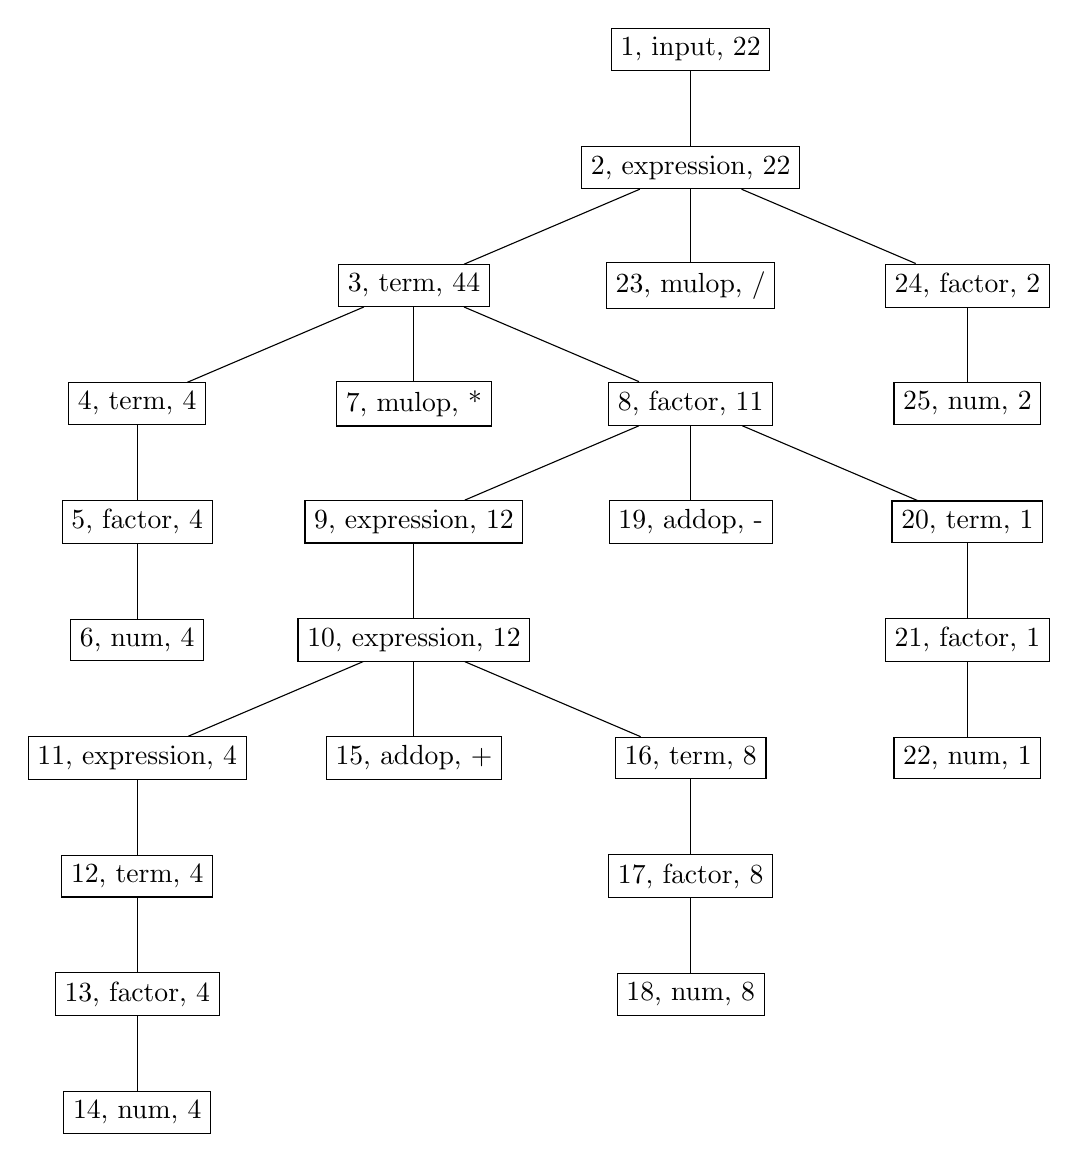
\begin{tikzpicture}[rectangle, sibling distance=100pt]
            \node[draw] {1, input, 22}
                child {node[draw] {2, expression, 22}
                    child {node[draw] {3, term, 44}
                        child {node[draw] {4, term, 4}
                            child{node[draw]{5, factor, 4}
                                child{node[draw]{6, num, 4}}
                            }
                        }
                        child{node[draw]{7, mulop, *}}
                        child{node[draw]{8, factor, 11}
                            child{node[draw]{9, expression, 12}
                                child{node[draw]{10, expression, 12}
                                    child{node[draw]{11, expression, 4}
                                        child{node[draw]{12, term, 4}
                                            child{node[draw]{13, factor, 4}
                                                child{node[draw]{14, num, 4}}
                                            }
                                        }
                                    }
                                    child{node[draw]{15, addop, +}}
                                    child{node[draw]{16, term, 8}
                                        child{node[draw]{17, factor, 8}
                                            child{node[draw]{18, num, 8}}
                                        }
                                    }
                                }
                            }
                            child{node[draw]{19, addop, -}}
                            child{node[draw]{20, term, 1}
                                child{node[draw]{21, factor, 1}
                                    child{node[draw]{22, num, 1}}
                                }
                            }
                        }
                    }
                    child {node[draw] {23, mulop, /}}
                    child {node[draw] {24, factor, 2}
                        child {node[draw] {25, num, 2}}
                    }
                }
            ;
        \end{tikzpicture}

        节点的编号即为示例代码在用访问者模式遍历该语法树时访问者到达语法树节点的顺序
\end{enumerate}

\end{sloppypar}
\end{document}